\documentclass{article} 
 \usepackage{graphicx}
 \begin{document} 

 \begin{tiny} 
Burn-In fraction = 0.100000
\textbf{ Chain Number = 1} 
\begin{center} 
 \begin{tabular}{ | c | c | c | c |} 
\hline parameter & $-\sigma$ & central & $+\sigma$ \\ 
 \hline 
sigma\_t\_ch & 0.896 & 0.931 & 0.971 \\ 
 sigma\_s\_ch & 0.911 & 1 & 1.11 \\ 
 sigma\_tW\_ch & 0.849 & 0.976 & 1.12 \\ 
 sigma\_ttbar & 1.11 & 1.16 & 1.2 \\ 
 sigma\_Diboson & 0.816 & 0.994 & 1.2 \\ 
 sigma\_DY & 0.875 & 1.07 & 1.3 \\ 
 sigma\_WQQ & 0.663 & 0.855 & 1.09 \\ 
 sigma\_Wc & 0.703 & 0.913 & 1.18 \\ 
 sigma\_Wb & 0.707 & 0.901 & 1.13 \\ 
 sigma\_Wother & 1.16 & 1.4 & 1.66 \\ 
 sigma\_Wlight & 0.81 & 1.04 & 1.31 \\ 
 sigma\_QCD & 0.755 & 1.6 & 3.2 \\ 
 lumi & 0.979 & 1 & 1.03 \\ 
 jes & -0.403 & 0.496 & 1.44 \\ 
 lf & -1.37 & -0.755 & -0.136 \\ 
 hf & -1.15 & -0.401 & 0.331 \\ 
 hfstats1 & -0.791 & 0.185 & 1.15 \\ 
 hfstats2 & -0.815 & 0.168 & 1.15 \\ 
 lfstats1 & -0.933 & 0.0479 & 1.04 \\ 
 lfstats2 & -1.03 & -0.0623 & 0.911 \\ 
 cferr1 & -0.0577 & 0.57 & 1.33 \\ 
 cferr2 & -0.105 & 0.683 & 1.55 \\ 
 PileUp & -0.115 & 0.467 & 1.12 \\ 
 pdf & -1.68 & -0.797 & 0.0907 \\ 
 LepId & -1.07 & -0.0819 & 0.888 \\ 
 LepTrig & -1.2 & -0.227 & 0.762 \\ 
 LepIso & -0.988 & 0.0253 & 1.01 \\ 
 Fac & -1.09 & -0.316 & 0.431 \\ 
 Ren & -4.31 & -3.5 & -2.68 \\ 
 RenFac & -5.23 & -4.55 & -3.87 \\ 
  \hline \end{tabular} 
 \end{center} 
\begin{center} 
 \begin{tabular}{ | c | c | c |} 
 \hline parameter & 95 \% UL & 98 \% UL \\ 
 \hline 
 7+8 TeV branching KU obs (exp) & 2.0 (2.8) \times 10^{-5} & \\ 
 7+8 TeV branching KC obs (exp) & 4.1 (2.8) \times 10^{-4} & \\ 
 \hline \end{tabular} 
 \end{center} 

 \newpage 

 \textbf{BURN IN STUDY} \\ 
 \includegraphics[width=0.9\linewidth]{BurnInStudysmTheta\_chain\_1.png} 
 \newpage 

 \textbf{COVARIANCE TABLE} \\ 
 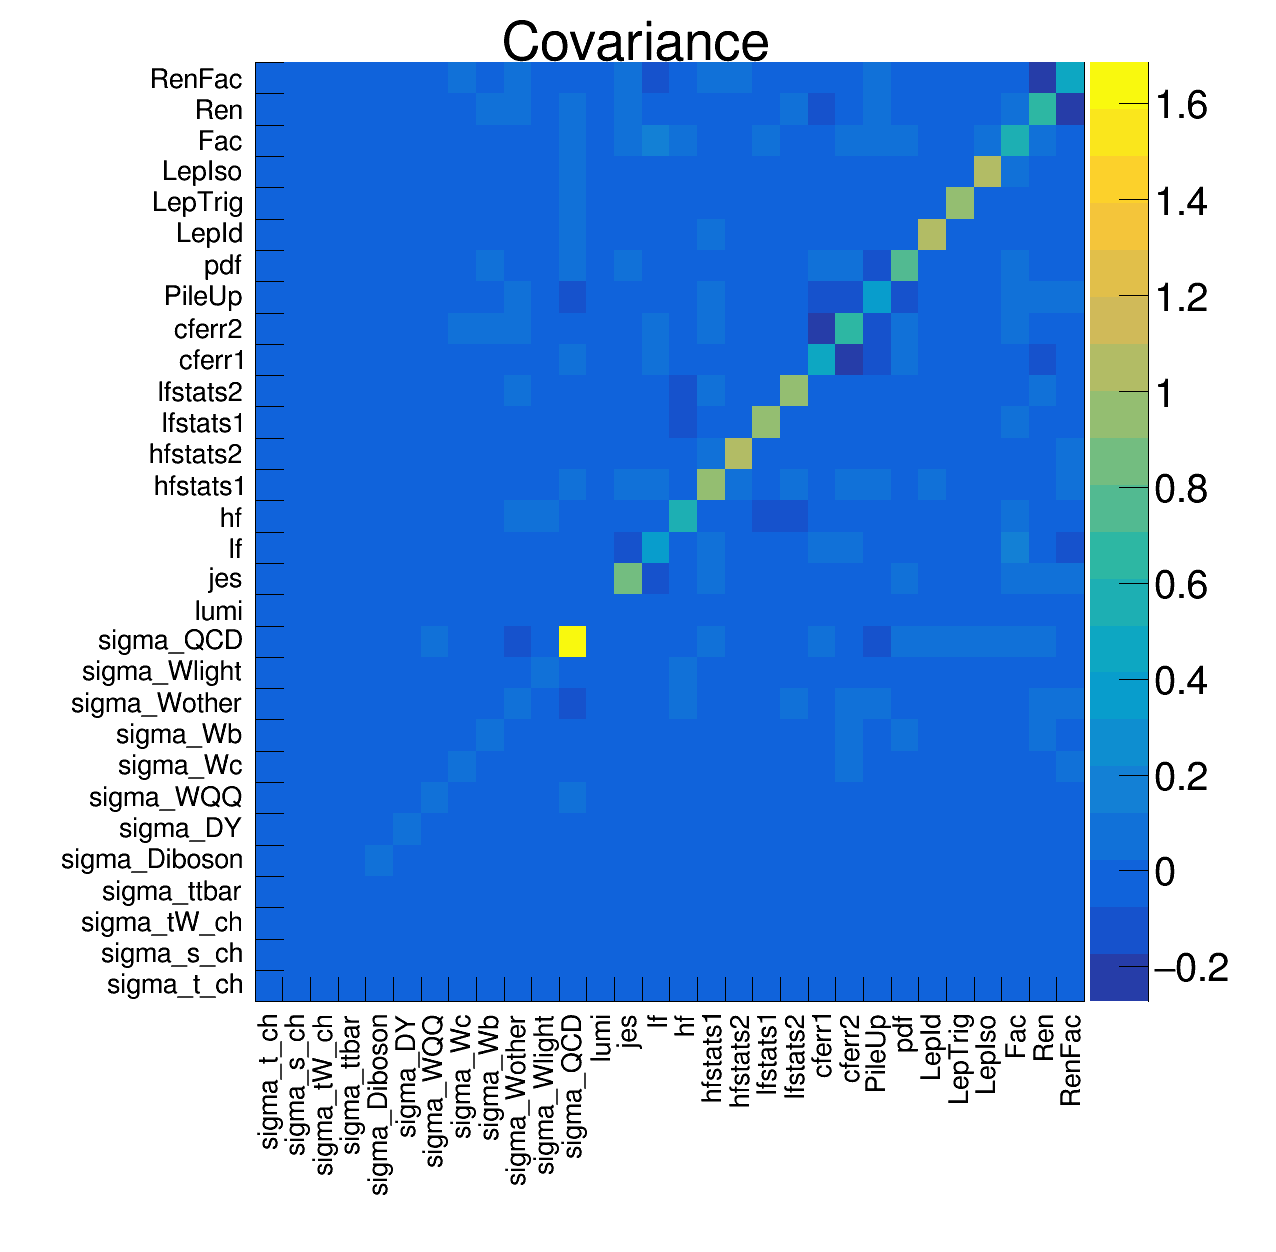
\includegraphics[width=0.7\linewidth]{Covsm.png} 
 \\ \textbf{CORRELATION TABLE} \\ 
 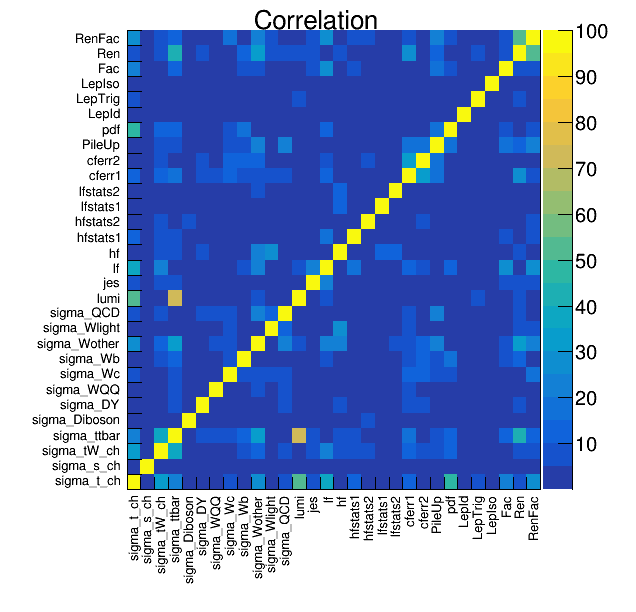
\includegraphics[width=0.7\linewidth]{Corsm.png} 
 \newpage 

 \textbf{MCMC OUTPUT CHAINS} \\ 
 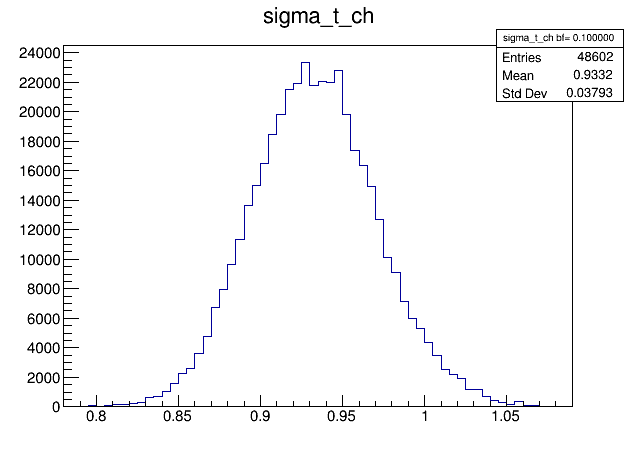
\includegraphics[width=0.33\linewidth]{chainsXsm/sigmaXtXchXsm.png}    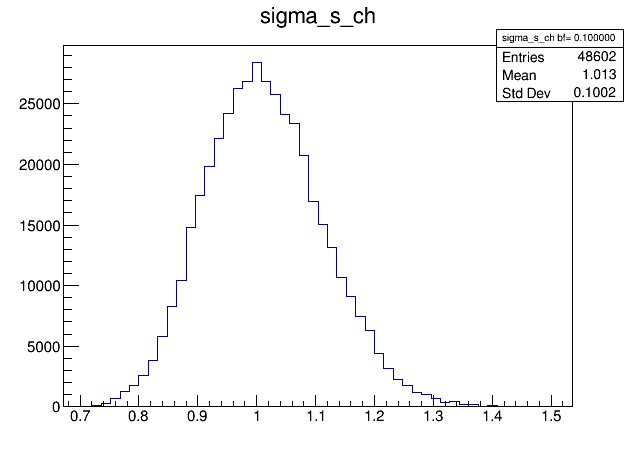
\includegraphics[width=0.33\linewidth]{chainsXsm/sigmaXsXchXsm.png}    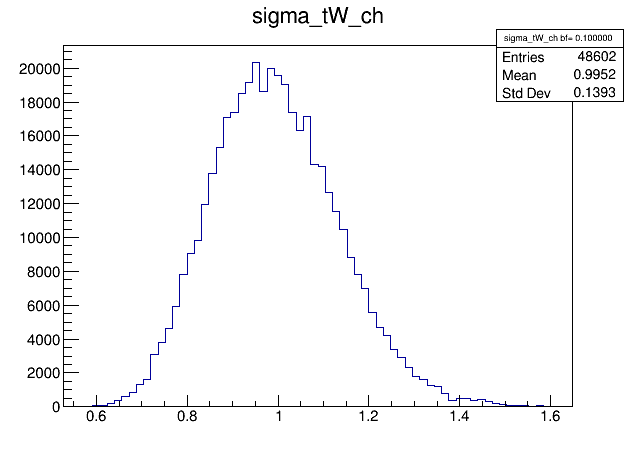
\includegraphics[width=0.33\linewidth]{chainsXsm/sigmaXtWXchXsm.png}  \ \ 
  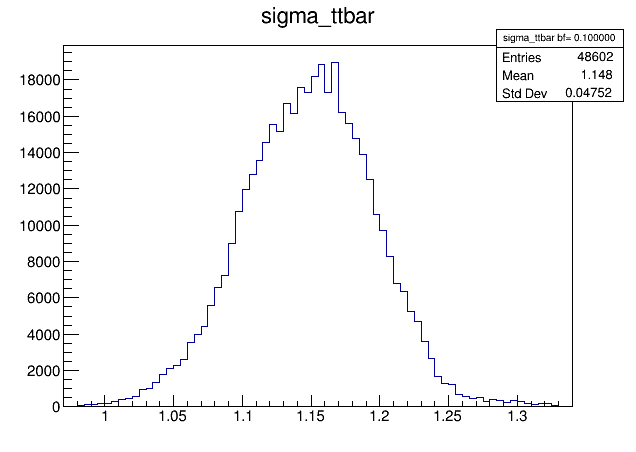
\includegraphics[width=0.33\linewidth]{chainsXsm/sigmaXttbarXsm.png}    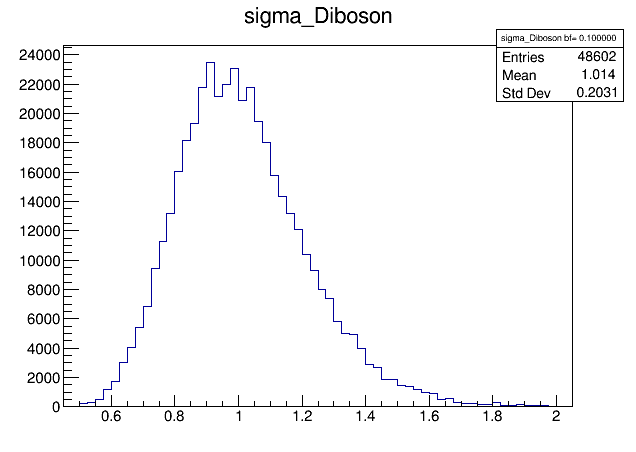
\includegraphics[width=0.33\linewidth]{chainsXsm/sigmaXDibosonXsm.png}  \ \ 
  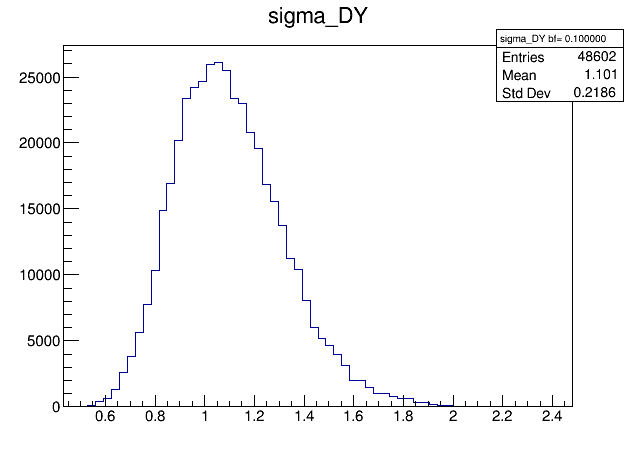
\includegraphics[width=0.33\linewidth]{chainsXsm/sigmaXDYXsm.png}    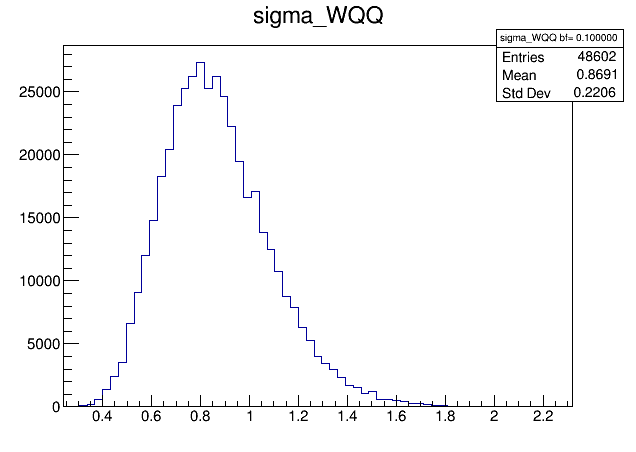
\includegraphics[width=0.33\linewidth]{chainsXsm/sigmaXWQQXsm.png}  \ \ 
  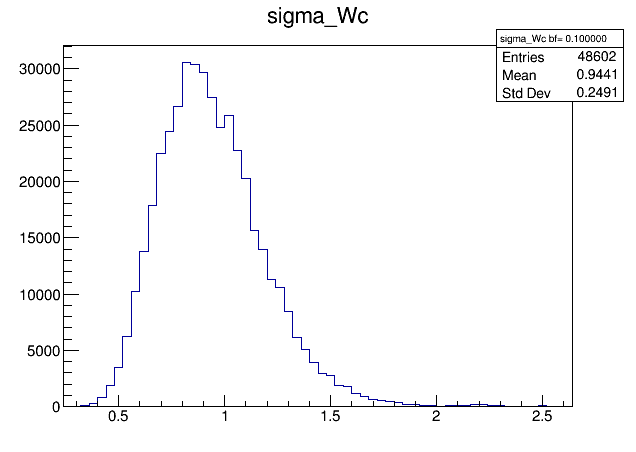
\includegraphics[width=0.33\linewidth]{chainsXsm/sigmaXWcXsm.png}    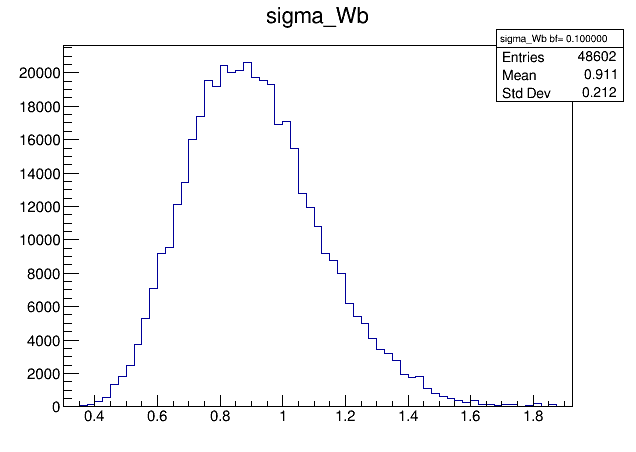
\includegraphics[width=0.33\linewidth]{chainsXsm/sigmaXWbXsm.png}  \ \ 
  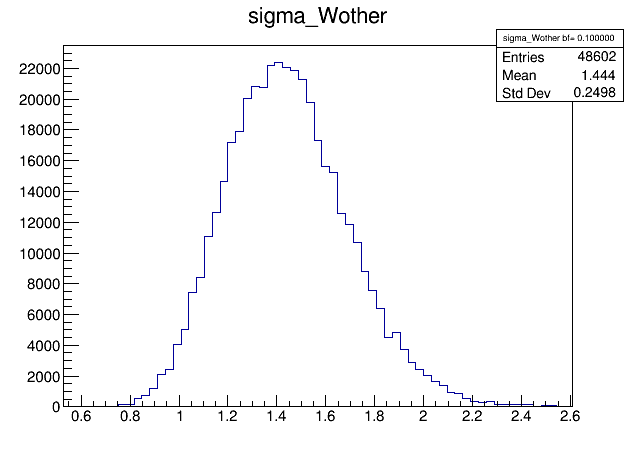
\includegraphics[width=0.33\linewidth]{chainsXsm/sigmaXWotherXsm.png}    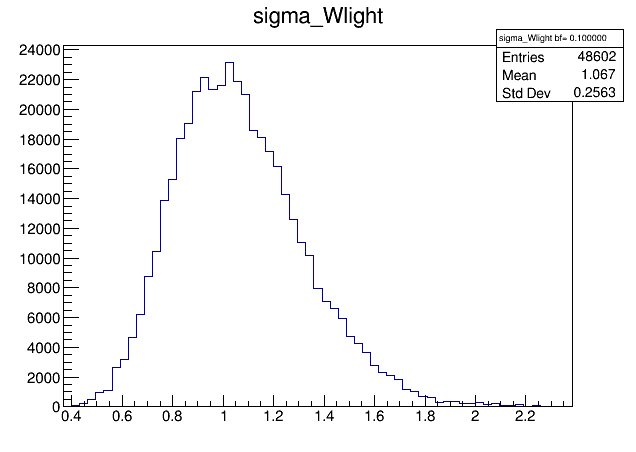
\includegraphics[width=0.33\linewidth]{chainsXsm/sigmaXWlightXsm.png}  \ \ 
  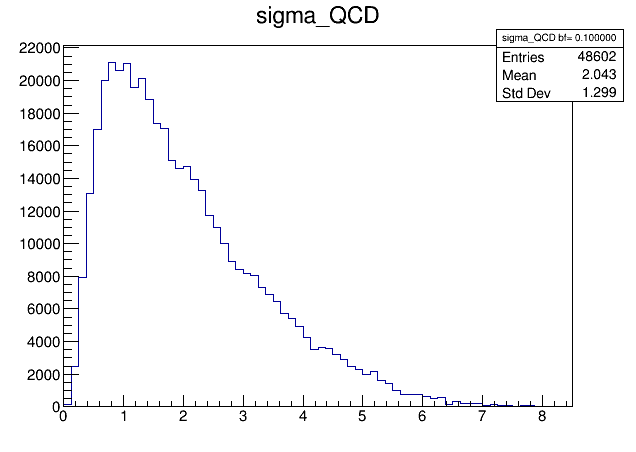
\includegraphics[width=0.33\linewidth]{chainsXsm/sigmaXQCDXsm.png}    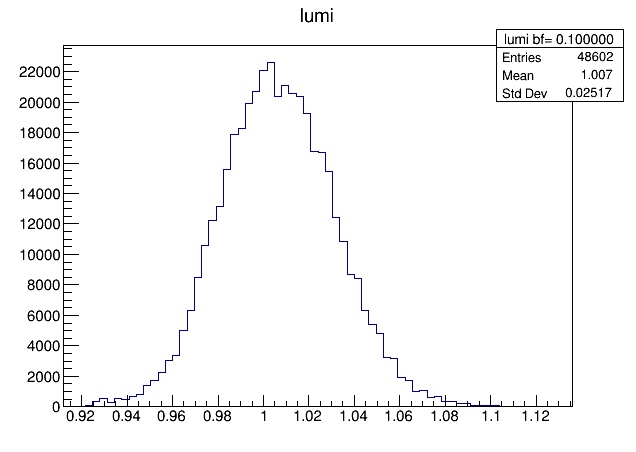
\includegraphics[width=0.33\linewidth]{chainsXsm/lumiXsm.png}  \ \ 
  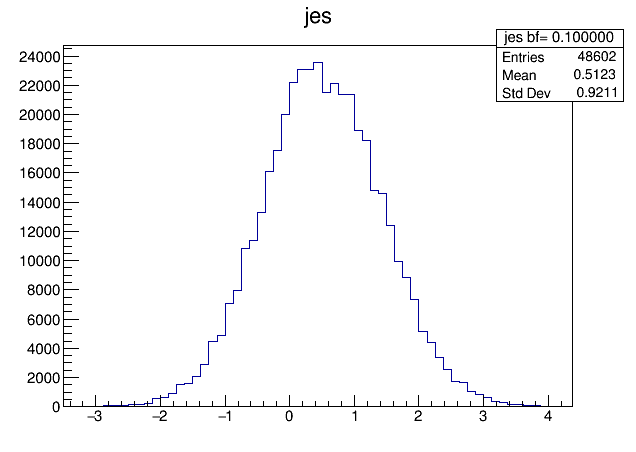
\includegraphics[width=0.33\linewidth]{chainsXsm/jesXsm.png}    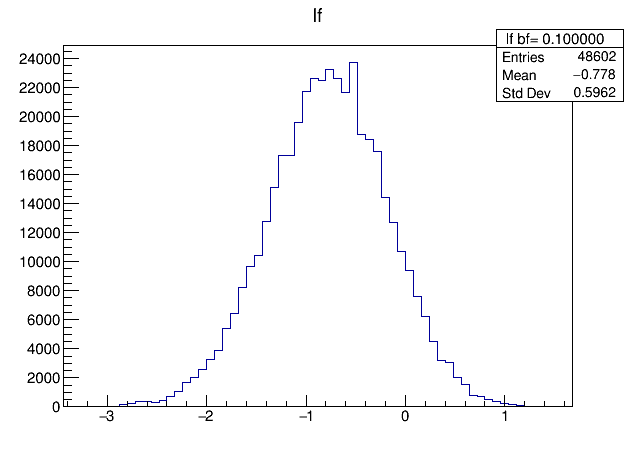
\includegraphics[width=0.33\linewidth]{chainsXsm/lfXsm.png}  \ \ 
  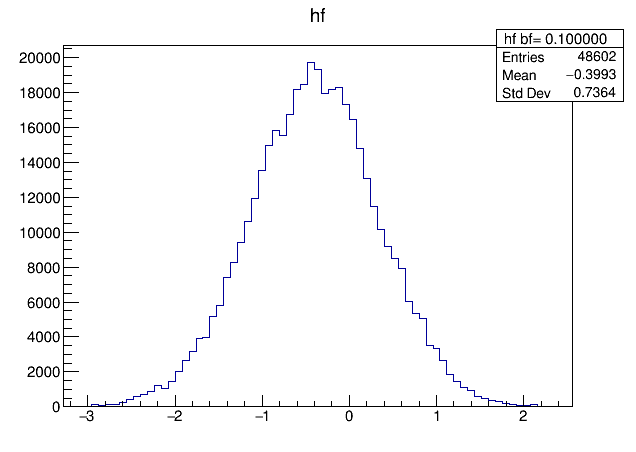
\includegraphics[width=0.33\linewidth]{chainsXsm/hfXsm.png}    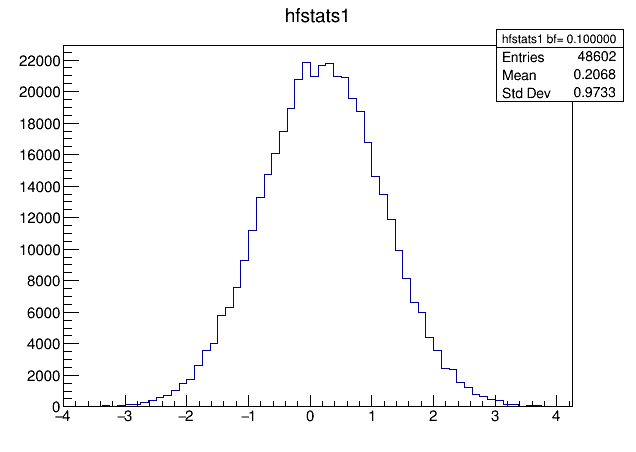
\includegraphics[width=0.33\linewidth]{chainsXsm/hfstats1Xsm.png}  \ \ 
  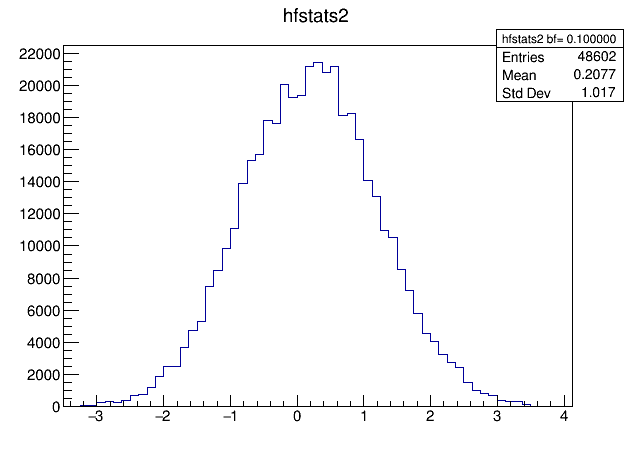
\includegraphics[width=0.33\linewidth]{chainsXsm/hfstats2Xsm.png}    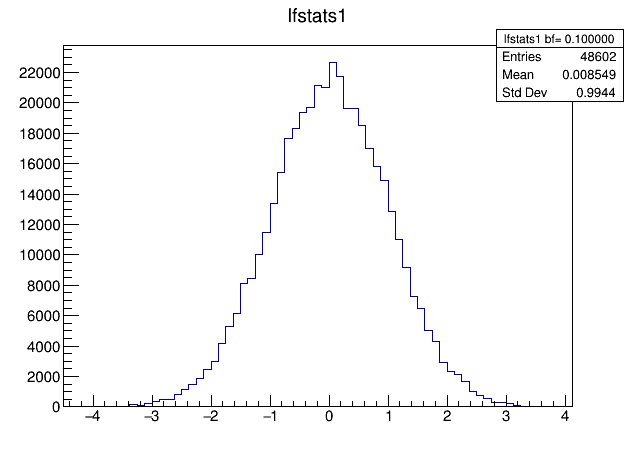
\includegraphics[width=0.33\linewidth]{chainsXsm/lfstats1Xsm.png}  \ \ 
  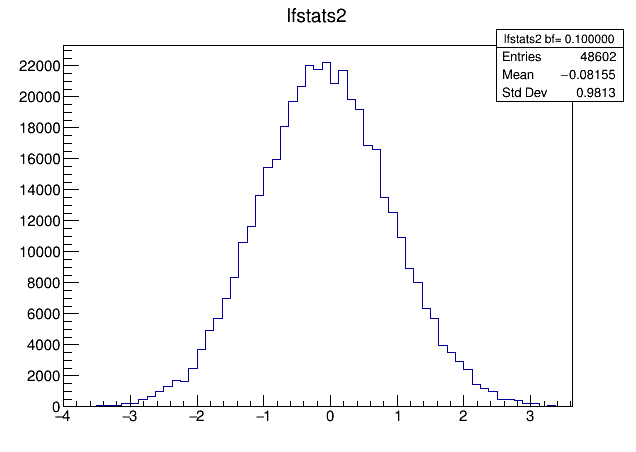
\includegraphics[width=0.33\linewidth]{chainsXsm/lfstats2Xsm.png}    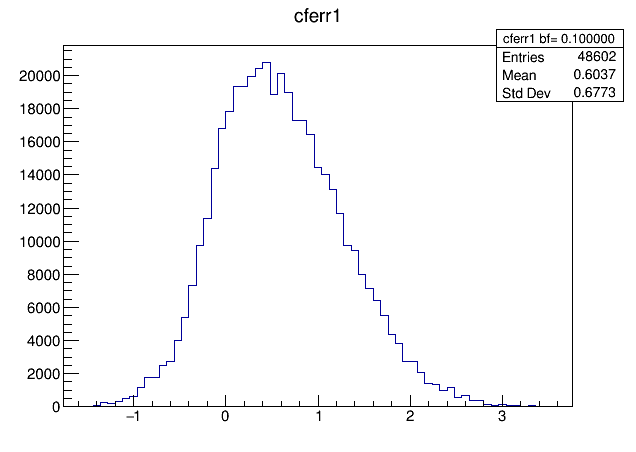
\includegraphics[width=0.33\linewidth]{chainsXsm/cferr1Xsm.png}  \ \ 
  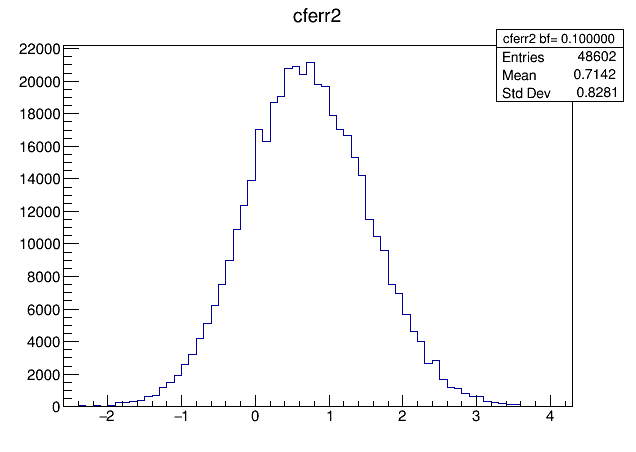
\includegraphics[width=0.33\linewidth]{chainsXsm/cferr2Xsm.png}    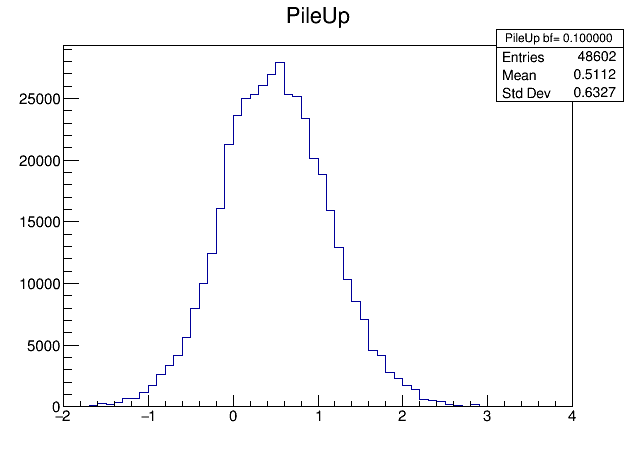
\includegraphics[width=0.33\linewidth]{chainsXsm/PileUpXsm.png}  \ \ 
  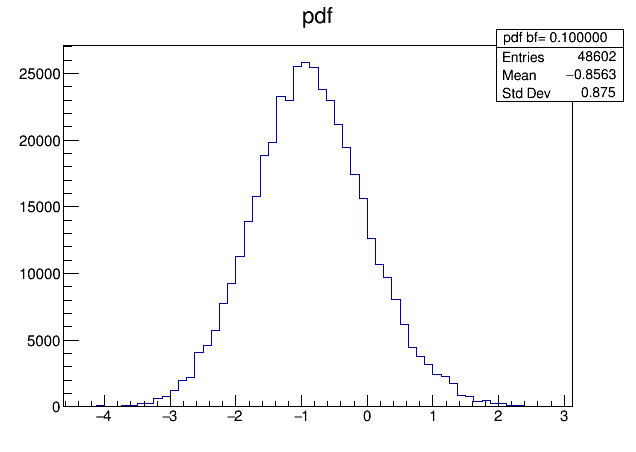
\includegraphics[width=0.33\linewidth]{chainsXsm/pdfXsm.png}    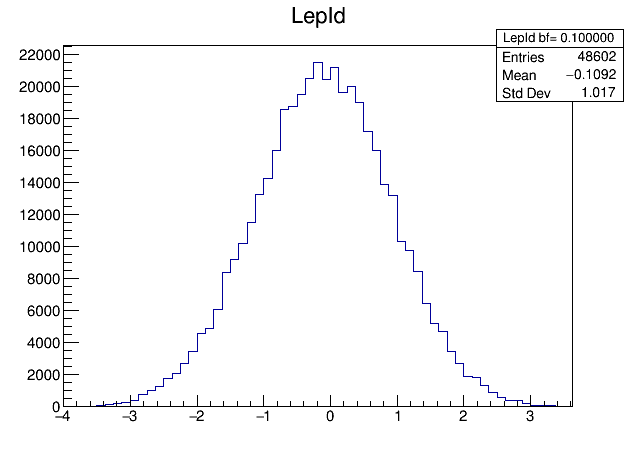
\includegraphics[width=0.33\linewidth]{chainsXsm/LepIdXsm.png}  \ \ 
  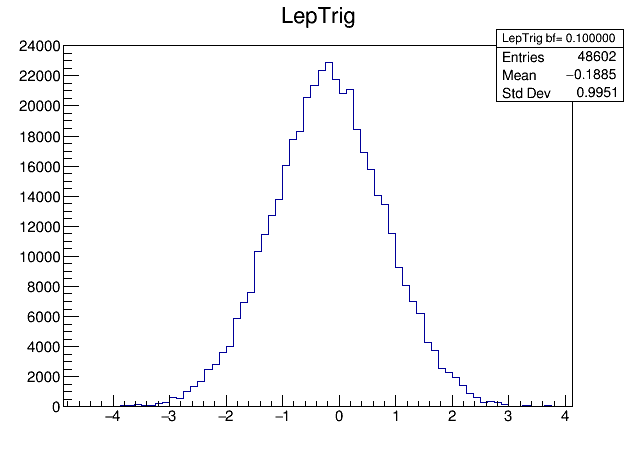
\includegraphics[width=0.33\linewidth]{chainsXsm/LepTrigXsm.png}    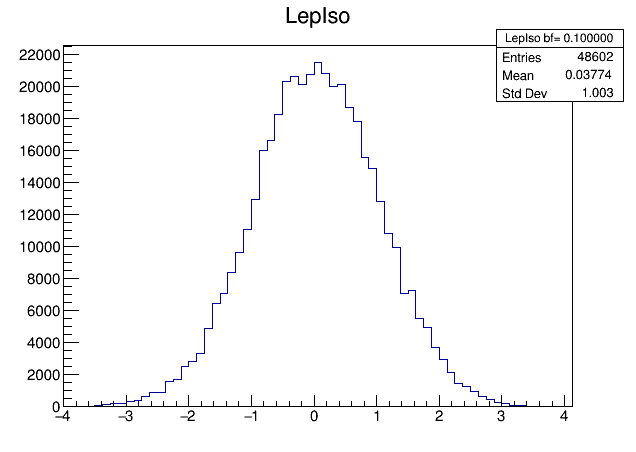
\includegraphics[width=0.33\linewidth]{chainsXsm/LepIsoXsm.png}  \ \ 
  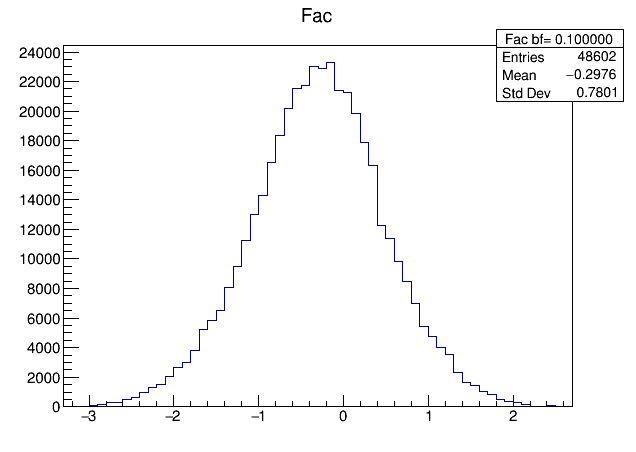
\includegraphics[width=0.33\linewidth]{chainsXsm/FacXsm.png}    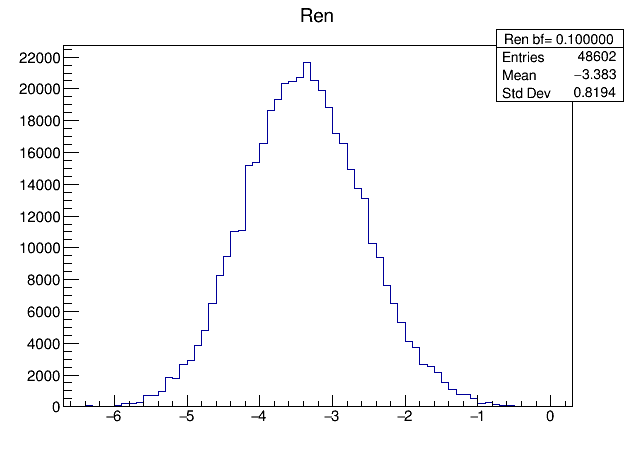
\includegraphics[width=0.33\linewidth]{chainsXsm/RenXsm.png}  \ \ 
  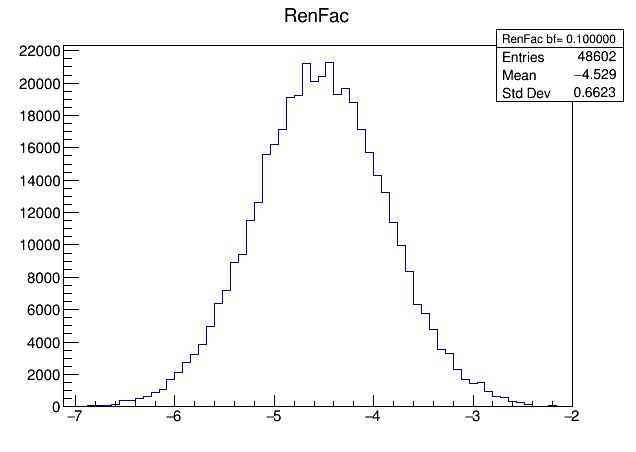
\includegraphics[width=0.33\linewidth]{chainsXsm/RenFacXsm.png}   
 \newpage 
\textbf{ Chain Number = 2} 
\begin{center} 
 \begin{tabular}{ | c | c | c | c |} 
\hline parameter & $-\sigma$ & central & $+\sigma$ \\ 
 \hline 
sigma\_t\_ch & 0.898 & 0.935 & 0.973 \\ 
 sigma\_s\_ch & 0.919 & 1.02 & 1.12 \\ 
 sigma\_tW\_ch & 0.858 & 0.99 & 1.13 \\ 
 sigma\_ttbar & 1.1 & 1.15 & 1.19 \\ 
 sigma\_Diboson & 0.822 & 0.994 & 1.21 \\ 
 sigma\_DY & 0.886 & 1.08 & 1.3 \\ 
 sigma\_WQQ & 0.654 & 0.846 & 1.09 \\ 
 sigma\_Wc & 0.706 & 0.91 & 1.17 \\ 
 sigma\_Wb & 0.706 & 0.89 & 1.11 \\ 
 sigma\_Wother & 1.21 & 1.45 & 1.7 \\ 
 sigma\_Wlight & 0.816 & 1.04 & 1.32 \\ 
 sigma\_QCD & 0.79 & 1.68 & 3.33 \\ 
 lumi & 0.98 & 1.01 & 1.03 \\ 
 jes & -0.393 & 0.498 & 1.43 \\ 
 lf & -1.38 & -0.764 & -0.144 \\ 
 hf & -1.15 & -0.436 & 0.281 \\ 
 hfstats1 & -0.77 & 0.248 & 1.25 \\ 
 hfstats2 & -0.753 & 0.228 & 1.22 \\ 
 lfstats1 & -0.946 & 0.0513 & 1.07 \\ 
 lfstats2 & -1.11 & -0.102 & 0.88 \\ 
 cferr1 & -0.12 & 0.504 & 1.25 \\ 
 cferr2 & -0.0905 & 0.725 & 1.59 \\ 
 PileUp & -0.0625 & 0.507 & 1.16 \\ 
 pdf & -1.74 & -0.912 & -0.0477 \\ 
 LepId & -1.11 & -0.131 & 0.867 \\ 
 LepTrig & -1.21 & -0.211 & 0.786 \\ 
 LepIso & -0.95 & 0.0337 & 1.07 \\ 
 Fac & -1.02 & -0.257 & 0.466 \\ 
 Ren & -4.18 & -3.35 & -2.58 \\ 
 RenFac & -5.18 & -4.51 & -3.83 \\ 
  \hline \end{tabular} 
 \end{center} 
\begin{center} 
 \begin{tabular}{ | c | c | c |} 
 \hline parameter & 95 \% UL & 98 \% UL \\ 
 \hline 
 7+8 TeV branching KU obs (exp) & 2.0 (2.8) \times 10^{-5} & \\ 
 7+8 TeV branching KC obs (exp) & 4.1 (2.8) \times 10^{-4} & \\ 
 \hline \end{tabular} 
 \end{center} 

 \newpage 

 \textbf{BURN IN STUDY} \\ 
 \includegraphics[width=0.9\linewidth]{BurnInStudysmTheta\_chain\_2.png} 
 \newpage 

 \textbf{COVARIANCE TABLE} \\ 
 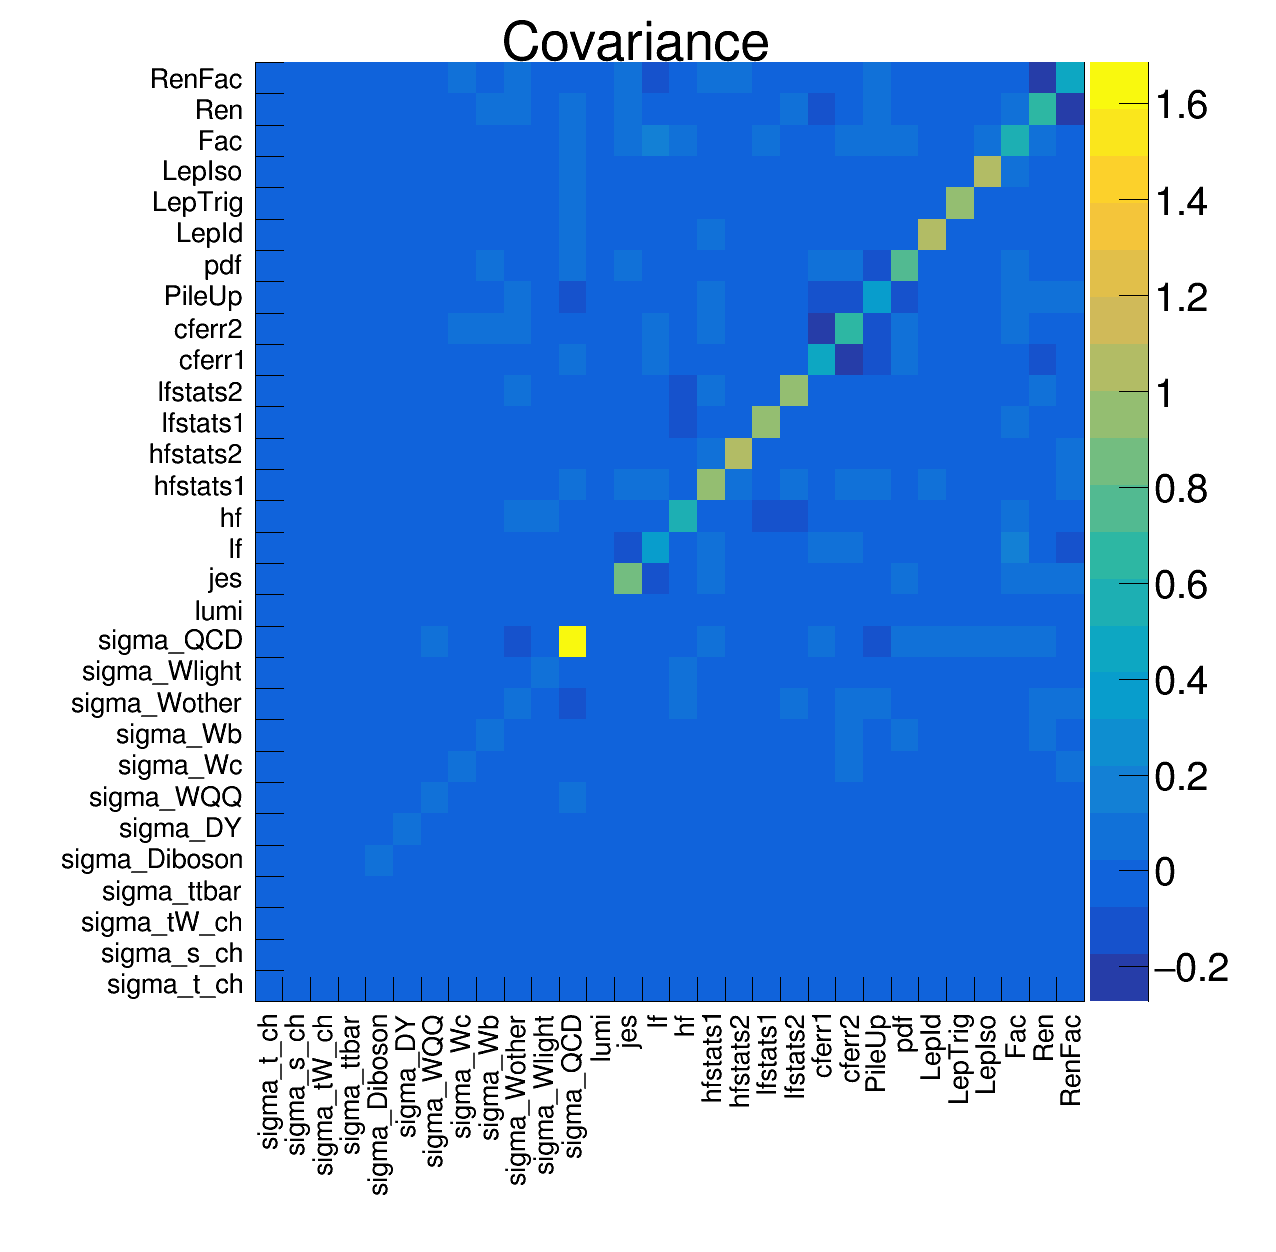
\includegraphics[width=0.7\linewidth]{Covsm.png} 
 \\ \textbf{CORRELATION TABLE} \\ 
 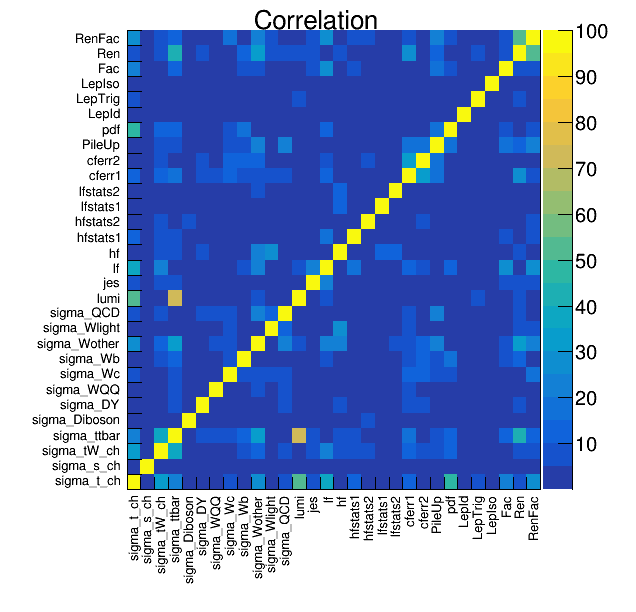
\includegraphics[width=0.7\linewidth]{Corsm.png} 
 \newpage 

 \textbf{MCMC OUTPUT CHAINS} \\ 
 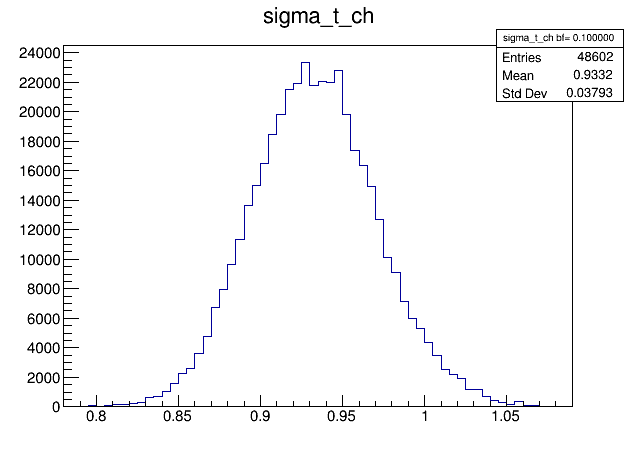
\includegraphics[width=0.33\linewidth]{chainsXsm/sigmaXtXchXsm.png}    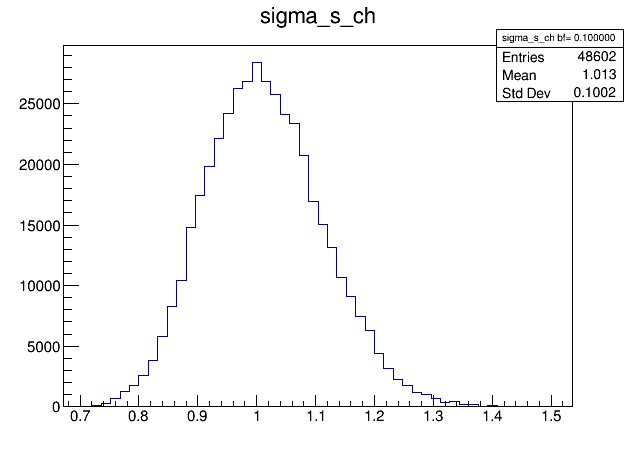
\includegraphics[width=0.33\linewidth]{chainsXsm/sigmaXsXchXsm.png}    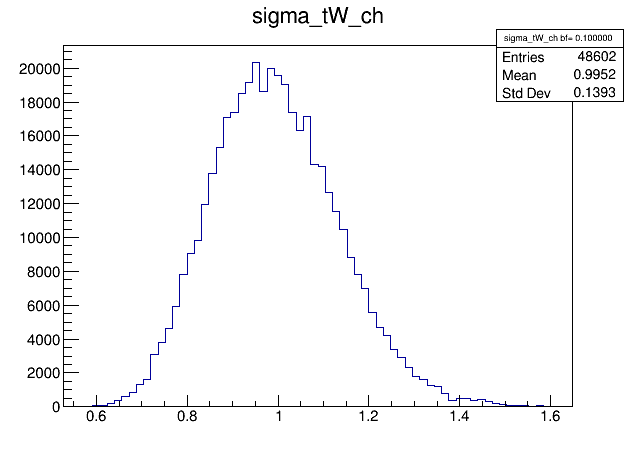
\includegraphics[width=0.33\linewidth]{chainsXsm/sigmaXtWXchXsm.png}  \ \ 
  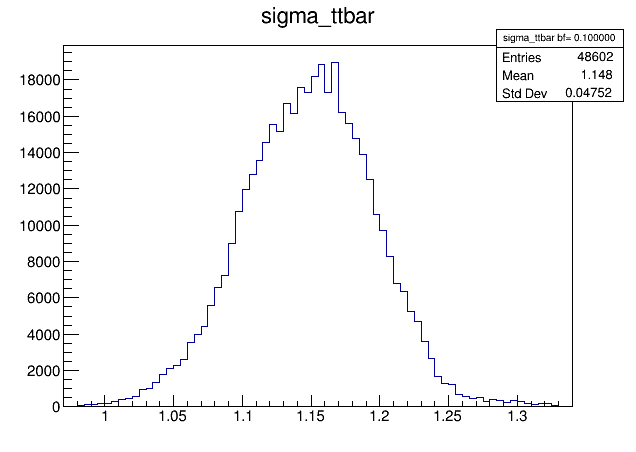
\includegraphics[width=0.33\linewidth]{chainsXsm/sigmaXttbarXsm.png}    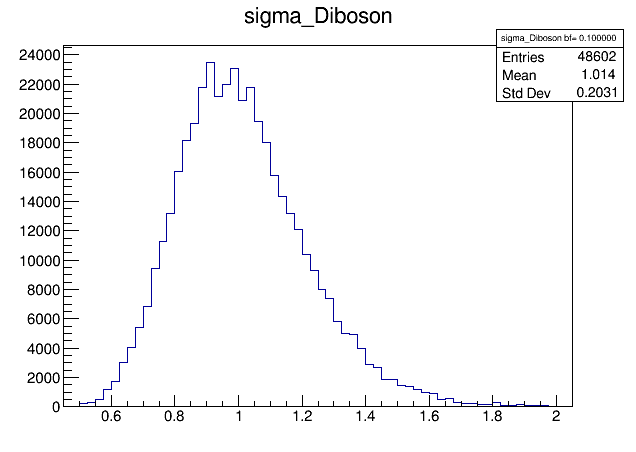
\includegraphics[width=0.33\linewidth]{chainsXsm/sigmaXDibosonXsm.png}  \ \ 
  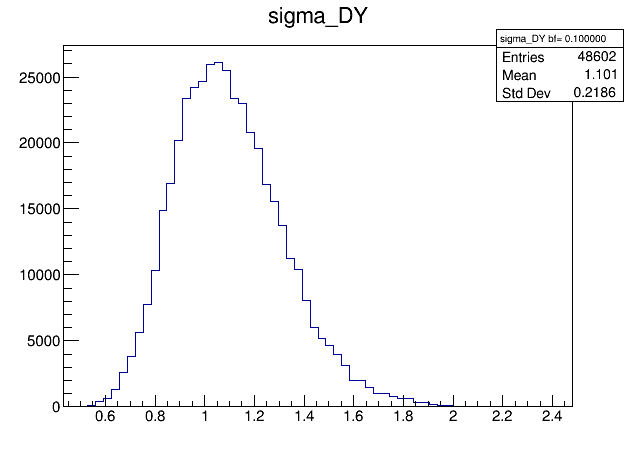
\includegraphics[width=0.33\linewidth]{chainsXsm/sigmaXDYXsm.png}    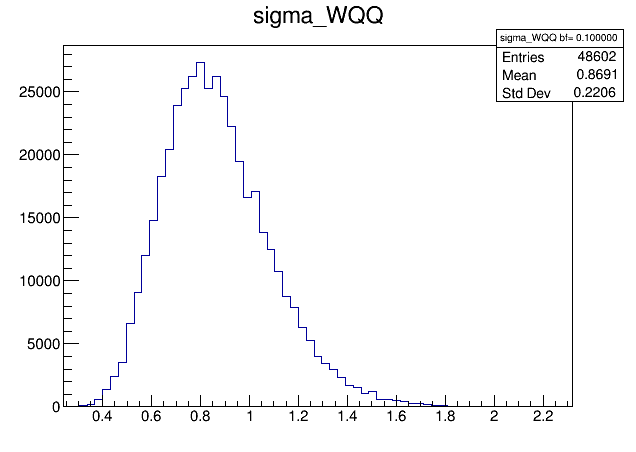
\includegraphics[width=0.33\linewidth]{chainsXsm/sigmaXWQQXsm.png}  \ \ 
  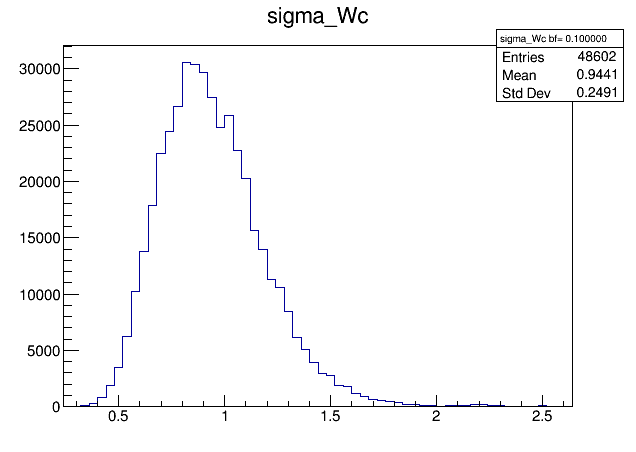
\includegraphics[width=0.33\linewidth]{chainsXsm/sigmaXWcXsm.png}    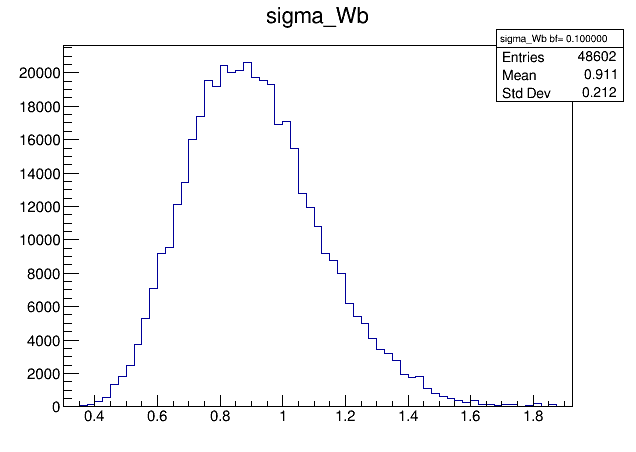
\includegraphics[width=0.33\linewidth]{chainsXsm/sigmaXWbXsm.png}  \ \ 
  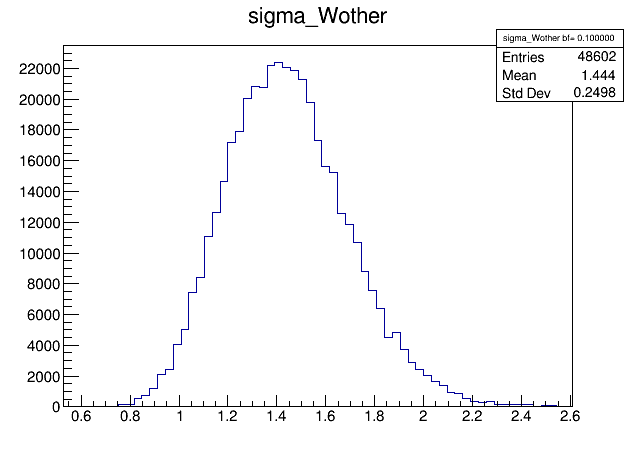
\includegraphics[width=0.33\linewidth]{chainsXsm/sigmaXWotherXsm.png}    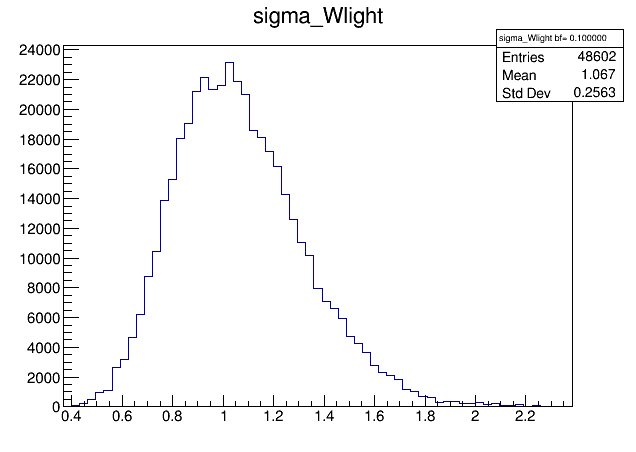
\includegraphics[width=0.33\linewidth]{chainsXsm/sigmaXWlightXsm.png}  \ \ 
  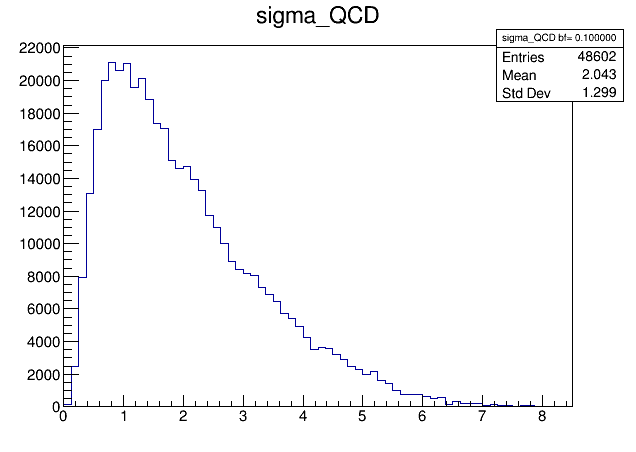
\includegraphics[width=0.33\linewidth]{chainsXsm/sigmaXQCDXsm.png}    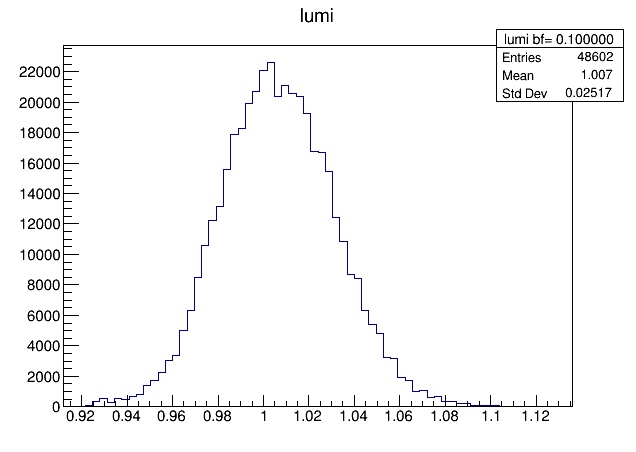
\includegraphics[width=0.33\linewidth]{chainsXsm/lumiXsm.png}  \ \ 
  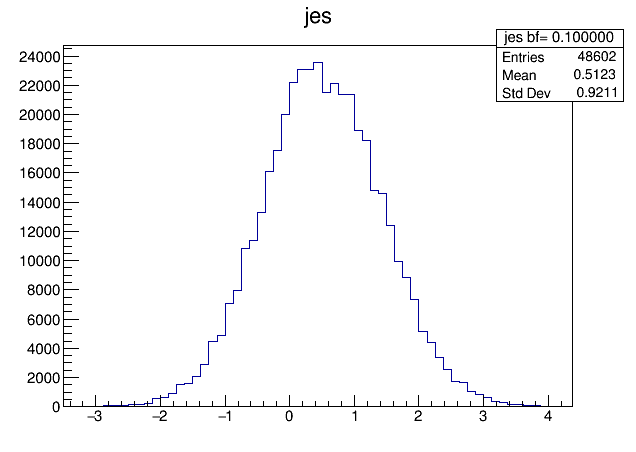
\includegraphics[width=0.33\linewidth]{chainsXsm/jesXsm.png}    \includegraphics[width=0.33\linewidth]{chainsXsm/lfXsm.png}  \ \ 
  \includegraphics[width=0.33\linewidth]{chainsXsm/hfXsm.png}    \includegraphics[width=0.33\linewidth]{chainsXsm/hfstats1Xsm.png}  \ \ 
  \includegraphics[width=0.33\linewidth]{chainsXsm/hfstats2Xsm.png}    \includegraphics[width=0.33\linewidth]{chainsXsm/lfstats1Xsm.png}  \ \ 
  \includegraphics[width=0.33\linewidth]{chainsXsm/lfstats2Xsm.png}    \includegraphics[width=0.33\linewidth]{chainsXsm/cferr1Xsm.png}  \ \ 
  \includegraphics[width=0.33\linewidth]{chainsXsm/cferr2Xsm.png}    \includegraphics[width=0.33\linewidth]{chainsXsm/PileUpXsm.png}  \ \ 
  \includegraphics[width=0.33\linewidth]{chainsXsm/pdfXsm.png}    \includegraphics[width=0.33\linewidth]{chainsXsm/LepIdXsm.png}  \ \ 
  \includegraphics[width=0.33\linewidth]{chainsXsm/LepTrigXsm.png}    \includegraphics[width=0.33\linewidth]{chainsXsm/LepIsoXsm.png}  \ \ 
  \includegraphics[width=0.33\linewidth]{chainsXsm/FacXsm.png}    \includegraphics[width=0.33\linewidth]{chainsXsm/RenXsm.png}  \ \ 
  \includegraphics[width=0.33\linewidth]{chainsXsm/RenFacXsm.png}   
 \newpage 
\textbf{ Chain Number = 3} 
\begin{center} 
 \begin{tabular}{ | c | c | c | c |} 
\hline parameter & $-\sigma$ & central & $+\sigma$ \\ 
 \hline 
sigma\_t\_ch & 0.895 & 0.932 & 0.97 \\ 
 sigma\_s\_ch & 0.913 & 1.01 & 1.11 \\ 
 sigma\_tW\_ch & 0.857 & 0.987 & 1.13 \\ 
 sigma\_ttbar & 1.1 & 1.15 & 1.19 \\ 
 sigma\_Diboson & 0.817 & 0.992 & 1.21 \\ 
 sigma\_DY & 0.886 & 1.08 & 1.32 \\ 
 sigma\_WQQ & 0.655 & 0.845 & 1.08 \\ 
 sigma\_Wc & 0.704 & 0.914 & 1.18 \\ 
 sigma\_Wb & 0.702 & 0.893 & 1.12 \\ 
 sigma\_Wother & 1.19 & 1.43 & 1.69 \\ 
 sigma\_Wlight & 0.817 & 1.04 & 1.32 \\ 
 sigma\_QCD & 0.799 & 1.74 & 3.39 \\ 
 lumi & 0.982 & 1.01 & 1.03 \\ 
 jes & -0.401 & 0.491 & 1.43 \\ 
 lf & -1.37 & -0.769 & -0.186 \\ 
 hf & -1.13 & -0.395 & 0.331 \\ 
 hfstats1 & -0.768 & 0.204 & 1.18 \\ 
 hfstats2 & -0.81 & 0.215 & 1.22 \\ 
 lfstats1 & -0.98 & 0.0155 & 1 \\ 
 lfstats2 & -1.06 & -0.0907 & 0.9 \\ 
 cferr1 & -0.0595 & 0.55 & 1.29 \\ 
 cferr2 & -0.103 & 0.698 & 1.54 \\ 
 PileUp & -0.0957 & 0.498 & 1.13 \\ 
 pdf & -1.72 & -0.883 & 0.0007 \\ 
 LepId & -1.13 & -0.0989 & 0.909 \\ 
 LepTrig & -1.18 & -0.194 & 0.807 \\ 
 LepIso & -0.953 & 0.0391 & 1.03 \\ 
 Fac & -1.07 & -0.287 & 0.457 \\ 
 Ren & -4.2 & -3.4 & -2.57 \\ 
 RenFac & -5.19 & -4.53 & -3.87 \\ 
  \hline \end{tabular} 
 \end{center} 
\begin{center} 
 \begin{tabular}{ | c | c | c |} 
 \hline parameter & 95 \% UL & 98 \% UL \\ 
 \hline 
 7+8 TeV branching KU obs (exp) & 2.0 (2.8) \times 10^{-5} & \\ 
 7+8 TeV branching KC obs (exp) & 4.1 (2.8) \times 10^{-4} & \\ 
 \hline \end{tabular} 
 \end{center} 

 \newpage 

 \textbf{BURN IN STUDY} \\ 
 \includegraphics[width=0.9\linewidth]{BurnInStudysmTheta\_chain\_3.png} 
 \newpage 

 \textbf{COVARIANCE TABLE} \\ 
 \includegraphics[width=0.7\linewidth]{Covsm.png} 
 \\ \textbf{CORRELATION TABLE} \\ 
 \includegraphics[width=0.7\linewidth]{Corsm.png} 
 \newpage 

 \textbf{MCMC OUTPUT CHAINS} \\ 
 \includegraphics[width=0.33\linewidth]{chainsXsm/sigmaXtXchXsm.png}    \includegraphics[width=0.33\linewidth]{chainsXsm/sigmaXsXchXsm.png}    \includegraphics[width=0.33\linewidth]{chainsXsm/sigmaXtWXchXsm.png}  \ \ 
  \includegraphics[width=0.33\linewidth]{chainsXsm/sigmaXttbarXsm.png}    \includegraphics[width=0.33\linewidth]{chainsXsm/sigmaXDibosonXsm.png}  \ \ 
  \includegraphics[width=0.33\linewidth]{chainsXsm/sigmaXDYXsm.png}    \includegraphics[width=0.33\linewidth]{chainsXsm/sigmaXWQQXsm.png}  \ \ 
  \includegraphics[width=0.33\linewidth]{chainsXsm/sigmaXWcXsm.png}    \includegraphics[width=0.33\linewidth]{chainsXsm/sigmaXWbXsm.png}  \ \ 
  \includegraphics[width=0.33\linewidth]{chainsXsm/sigmaXWotherXsm.png}    \includegraphics[width=0.33\linewidth]{chainsXsm/sigmaXWlightXsm.png}  \ \ 
  \includegraphics[width=0.33\linewidth]{chainsXsm/sigmaXQCDXsm.png}    \includegraphics[width=0.33\linewidth]{chainsXsm/lumiXsm.png}  \ \ 
  \includegraphics[width=0.33\linewidth]{chainsXsm/jesXsm.png}    \includegraphics[width=0.33\linewidth]{chainsXsm/lfXsm.png}  \ \ 
  \includegraphics[width=0.33\linewidth]{chainsXsm/hfXsm.png}    \includegraphics[width=0.33\linewidth]{chainsXsm/hfstats1Xsm.png}  \ \ 
  \includegraphics[width=0.33\linewidth]{chainsXsm/hfstats2Xsm.png}    \includegraphics[width=0.33\linewidth]{chainsXsm/lfstats1Xsm.png}  \ \ 
  \includegraphics[width=0.33\linewidth]{chainsXsm/lfstats2Xsm.png}    \includegraphics[width=0.33\linewidth]{chainsXsm/cferr1Xsm.png}  \ \ 
  \includegraphics[width=0.33\linewidth]{chainsXsm/cferr2Xsm.png}    \includegraphics[width=0.33\linewidth]{chainsXsm/PileUpXsm.png}  \ \ 
  \includegraphics[width=0.33\linewidth]{chainsXsm/pdfXsm.png}    \includegraphics[width=0.33\linewidth]{chainsXsm/LepIdXsm.png}  \ \ 
  \includegraphics[width=0.33\linewidth]{chainsXsm/LepTrigXsm.png}    \includegraphics[width=0.33\linewidth]{chainsXsm/LepIsoXsm.png}  \ \ 
  \includegraphics[width=0.33\linewidth]{chainsXsm/FacXsm.png}    \includegraphics[width=0.33\linewidth]{chainsXsm/RenXsm.png}  \ \ 
  \includegraphics[width=0.33\linewidth]{chainsXsm/RenFacXsm.png}   
 \newpage 

 \newpage 

 \textbf{INPUT HISTOGRAMMS} \\ 

 \end{tiny} 
 
 \end{document} 

